% flatex input: [gnd_dn_lambda.tex]

\begin{figure}[h]
\centering
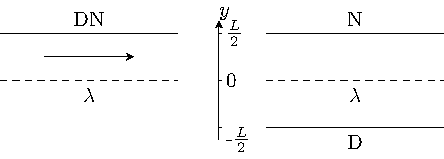
\includegraphics{fig_gnd_dn_lambda.pdf}
\caption{Partition function of Hamiltonian with DN and $\lambda$ boundary conditions. The width of the strip is $\pi$ due to folding. We unfold the cylinder and the new stripe have $N$ and $D$ boundary conditions on the left and right plus a $\lambda$ junction in the middle. }
\label{fig:Fig_gnd_dn_lambda}
\end{figure}

In this appendix, we would like to calculate the amplitude for the setup shown in Fig.~\ref{fig:Fig_gnd_dn_lambda}. In particular, the unfolded configuration has D/N boundary conditions at $x = \pm \frac{L}{2}$ and linking boundary condition at $x = 0$. The general solutions can be written as
\begin{equation}
\label{eq:normalized_f}
f(k, x) = 
\left\lbrace
\begin{aligned}
  A_1 e^{i kt} \cos\left(kx +\frac{1}{2}kL \right) &  \quad x < 0  \\
  A_2 e^{ikt}  \sin\left(kx - \frac{1}{2}kL \right) & \quad x > 0   \\
\end{aligned} \right. 
\end{equation}
As demonstrated in the {\bf\color{red}main text}, if we denote $f(k,x<0)\equiv\phi_1$ and $f(k,x>0)\equiv\phi_2$, the boundary condition at the junction reads
\begin{eqnarray}\begin{aligned}
\frac{\partial_x \phi_1}{ \partial_t \phi_1} = \lambda^2 \frac{\partial_x \phi_2}{ \partial_t \phi_2} = \tan^2 \theta\frac{\partial_x \phi_2}{ \partial_t \phi_2} \quad \theta \in \left[0,\frac{\pi}{2} \right]  
\end{aligned}\end{eqnarray}
which implies
\begin{equation}
\label{eq:momentum_gnd_dn_lambda}
k = \frac{2\pi}{L}\left( n \pm \frac{\theta}{\pi} \right)  \quad n\in\mathbb{Z}
\end{equation}
It is evident that the momentum $k$ is shifted from integer multiple of $2\pi/L$ due to the $\lambda$ boundary condition in the middle. 
\begin{comment}
Thus, the normalized eigenfunctions are
\begin{equation}
f_n(x) = \sqrt{\frac{2}{L}}
\left\lbrace
\begin{aligned}
  \cos(kx +\frac{1}{2}kL ) &  \quad x < 0  \\
  \pm \sin(kx - \frac{1}{2}kL ) & \quad x > 0   \\
\end{aligned} \right. 
\qquad 
k = \frac{2\pi}{L}\left( n \pm  \frac{\theta}{\pi} \right)  \quad n \in \mathbb{Z} 
\end{equation}
Expand the field $\phi = \sum_n \phi_n f_n(x) $, the action and Hamiltonian becomes
\begin{equation}
  S = \frac{g}{2} \int dt \, \sum_{n \in \mathbb{Z} }\left(  \dot{\phi}^2_n + k^2 \phi_n^2 \right) \implies\quad   g \dot{\phi}_n  = \pi_n \quad \implies H =  
\frac{1}{2g}\sum_{n \in \mathbb{Z} } \pi_n^2 + ( kg )^2  \phi_n^2 
\end{equation}
\end{comment}

It is clear that the normalized eigenfunctions in Eq.~\eqref{eq:normalized_f} serves as orthonormal basis in mode expansion. Following the same procedure in \onlinecite{di_francesco_conformal_1997}, we have the Hamiltonian as
\begin{equation}
\label{eq:H_in_gnd_dn_lambda}
H = \frac{1}{2} \sum_{n \in \mathbb{Z} } |k|  \left(a^{\dagger}_n a_n + \frac{1}{2} \right)
\end{equation}
where the momentum $k$ is defined in Eq.~\eqref{eq:momentum_gnd_dn_lambda}, and the creation and annihilation operators defined as usual
\begin{equation}
\begin{aligned}
a_n = \frac{1}{\sqrt{2}} \left( \sqrt{ |k|g} \phi_n + \frac{i }{\sqrt{|k|g} }\pi_n  \right) \\
a^{\dagger}_n = \frac{1}{\sqrt{2}} \left( \sqrt{ |k|g} \phi_n - \frac{i }{\sqrt{|k|g} }\pi_n  \right) \\
\end{aligned}
\end{equation}

The Casimir energy is the vacuum energy brought by the finite size of the setup. From Eq.~\eqref{eq:H_in_gnd_dn_lambda} and define $x\equiv\theta/\pi$ in Eq.~\eqref{eq:momentum_gnd_dn_lambda}, we have
\begin{equation}
\begin{aligned}
E_c &= \frac{1}{4} \sum_{n \in \mathbb{Z}} | k| = \frac{\pi}{2L} \left( \sum_{n \in \mathbb{Z}}  | n + x | + \sum_{n \in \mathbb{Z}}  | n - x |  \right) \\  
&= \frac{\pi}{L} \Big[\sum_{n \ge 0 } ( n + x )^{-s} + \sum_{n \ge 0 }  ( n - x)^{-s}  +   x^{-s} \Big]\Big|_{s = -1} \\
&= \frac{\pi}{L} \left[ \zeta_{\rm H}( -1, x ) + \zeta_{\rm H}( -1, x ) +  x \right] \\
&= \frac{1}{2} \left( - x^2 + x - \frac{1}{6}\right)
\end{aligned}
\end{equation}
where we used the fact that the unfolded geometry has length $L=2\pi$. Thus the free energy reads
\begin{equation}
F = \beta E_c = - \frac{\beta}{2} B_2( x) 
\end{equation}
which agrees with the boundary state calculation in Eq.{\bf\color{red}where}

